%!TEX root = kudzai_thesis.tex
%%%%%%%%%%%%%%%%%%%%%%%%%%%%%%%%%%%%%%%%%%%%%%%%%%%%%%%%%%%%%%%%%%%%%%%


\chapter{Problem Statement}
Mass demonstrations by people often result in vandalism of public property in industry, academia, etc., which leads to the disruption of daily organizational activities. They often use social media as a platform to express their views, sometimes extreme views towards the authorities. People’s opinions are very valuable information in decision making process. Nowadays several websites encourage users to express and exchange their views, suggestions and opinions related to textual content publically. The increase in popularity of these sites resulted in huge collection of peoples’ opinion on the web in much unstructured manner. Extracting the useful content from these opinion sources becomes a challenging task. Recent attempts to compute sentiment analysis on unstructured data have used techniques such as opinion mining, sentiment lexicon.

\section{Objectives}

\begin{itemize}
\item To detect people\textquotesingle s mood from textual information posted on social media.
\item To classify people\textquotesingle s sentiment based on their geographical location.
\end{itemize}

\section{Aim}

Our aim is to develop a system that can classify people\textquotesingle s mood and sentiment based on the textual information they post on social media.



\section{Significance of the Study}
Leaders of today face many difficult, potentially explosive situations in which they must make decisions that can help or harm their firms, themselves or others. Sentiment analysis will improve the ethical quality of decisions made by the authorities and managers, and also ensure that decisions made will not backfire. It also helps the authorities to predict the outcome of the decisions made, and determine the impact on the affected population. This study helps us to evaluate the degree of evaluability/argumentativeness with which the population under study communicates,\cite{ref5} and make improved decisions based on the analyzed data.



\chapter{Research methodology}

A graphical description of the processes involved in sentiment analysis approach that this research will follow is detailed in the diagram shown below,\cite{ref21}:

\begin{figure}[h]
  \centering
  \pgfimage[width=0.7\linewidth]{images/research_methodology}
  \caption[]
  {Processes involved in sentiment analysis}
  \label{fig:ALAP:sm3}
\end{figure}


\subsection{Data Collection}
Sentiment analysis takes advantage of the vast user generated content over the internet.
The data source points to queries of user discussions on public forums like blogs,
discussion boards and product reviews boards as well as on private logs through social
network sites like Twitter and Facebook. Very often, the data log is bulky, disorganized,
and disintegrated on multiple portals. Opinions and feelings are expressed in different ways
including the amount of details given, type of vocabulary used, context of writing, slangs
and lingua variations are just a few examples. This makes manual analysis tedious, and
almost impossible. But, with sentiment analysis, innovative text analytics and natural
language processing is employed to extract and classify data. Once the data is extracted, it
will then be prepared for analysis. An example of the data is presented below



\begin{figure}[h]
  \centering
  \pgfimage[width=0.8\linewidth]{images/sample_tweets}
  \caption[Example figure]%
  {sample tweets for cocacola: source (T. Nyamandi et al, 2015)}
  \label{fig:ALAP:sm1}
\end{figure}


\subsection{Text Preparation}
Text preparation involves cleaning the extracted data before the analysis is performed.
Usually text preparation involves identifying and eliminating non textual content from the
textual dataset, and any information that can reveal the identities of reviewers including:
reviewer name, reviewer location, review date. In addition, any other content that is not
deemed relevant to the area of study is also removed from the textual dataset such as
includes stop words or words that are not relevant to the course of analysis.

\subsection{Sentiment Detection}
The third stage is sentiment detection. Sentiment detection requires appraising and
extracting reviews and opinions from the textual dataset through the use of computational
tasks. Each sentence is examined for subjectivity. Only sentences with subjective
expressions are kept in the dataset. Sentences that convey facts and objective
communication are discarded from further analysis. Sentiment detection is done at different
levels either single term, phrases, complete sentences or complete document with
commonly used techniques such as:


\begin{itemize}

\item \textbf{Unigrams:} This is a classic approach where each element is represented as a feature
vector based on frequency of a single word. It is often described as a bag of words
approach.

\item \textbf{N-Grams:} In this approach the features of a document is represented by multiple words
in sequence (e.g.: words in pairs, triplets) which captures more context.

\item \textbf{Lemmas:} This involves the use of synonyms rather than the literal word. For example:
better $\xrightarrow{}$ good, best $\xrightarrow{}$ good. This method reportedly makes the classification task easier as well as facilitates generalization.

\item \textbf{Negation:} This is basically an extension to the n-gram methods where the phrases “I
like this book” and “I do not like this book” would have considered similar under most
classification techniques, but with negation, both terms are forced into opposite
groupings. However, negation is not always easy to model.
For instance,\cite{ref19}, reported that it is difficult to identify negation when
sarcasms and ironies are used in a sentence. Additionally, the negation term does not
always reverse the polarity.

\item \textbf{Opinion words:} These are basically words that are used to describe people feelings and
opinions (nouns, verbs, adjectives, adverbs). These words are incorporated into a
feature vector where they represent the presence of absence of a word. These words
are good indicators of subjectivity in a document.
\end{itemize}

\subsection{Sentiment Classification}
The fourth stage is polarity classification which classifies each subjective sentence in the
textual dataset into classification groups. Usually these groups are represented on two
extreme points on a continuum (positive, negative; good, bad; like, dislike). However,
classification can also involve multiple points similar to the star ratings used by hotels,
restaurants and retailers. The three basic functions under supervised learning available for
classification include: Naive Bayes (NB), Support Vector Machines (SVM) and Maximum
- Entropy (ME). A Naive Bayes classifier is a probabilistic classifier based on applying
Bayes’ theorem assuming that features are independent given the class label. This classifier
is constructed based on the frequency of occurrence of each feature per class in the training
data set. Support vector machines are based on the statistical learning theory,\cite{ref40}. Binary classifiers show high generalization capability by looking for a
hyper plane that maximizes the separation margin between observations from different
classes. The use of kernels allows their use for nonlinear problems. Under ME a number
of models are constructed where each feature correspond to a constraint on the model. The
model with the maximum entropy over all models is selected for classification.

\clearpage
\subsection{Presentation of Output}
The general purpose of the analysis is to convert unstructured fragmented text into
meaningful information. Once the analysis is completed, a number of conventional options
are used to display the result of text analysis, among them is the use of graphical
displays such as pie charts, bar charts and line graphs. The polarity is segmented on color,
frequencies, percentages and size. The format of presentation depends on the research
interest. Examples of each are shown below:

\begin{figure}[h]
  \centering
  \pgfimage[width=0.7\linewidth]{images/sentiment_summary}
  \caption[Vector graphics example]%
  {Sentiment summary on a single product.}
  \label{fig:ALAP:sm3}
\end{figure}


Our focus is on methods that seek to address the new challenges raised by sentiment-aware
applications, as compared to those that are already present in more traditional fact-based analysis


\section{Limitations}
Due to the limitations of the current information processing and analysis techniques ( i.e. search
engines cannot crawl and process pictures, video, flash, executive scripts, executive program and
other non-text content files ), images, videos, folders, executive files, package files and other
online transmission information and data are not included in our analysis, \cite{ref22}.


\leavevmode\\
When an unexpected geopolitical event occurs and spreads on the internet, the news reports and
comments on social media can objectively reflect the concerns and opinions of the citizens. But as it is difficult to do extensive gathering and analysis of ancillary data and theme
events information to reveal and explain the spatial diffusion of internet attention always be
blocked and insipid, \cite{ref22}. As a result, this study will use the web crawler
technology, and twitter API to gather textual information based on a geographic location, to detect moods
of a particular population on a certain topic.


\subsection{Delimitations of the study}
Although there may be value in studying all social network platforms and mass media sites, this study is limited to Twitter comments. A complicating factor for online sentiment detection is that there are many electronic communications media in which text-based communication in English seems to frequently ignore
the rules of grammar and spelling.


\section{Literature Review}
\subsection{Overview}
In this chapter we look at the available technologies as well as the progress that has been
made in the area of concern that is sentiment analysis. The researcher will discuss the work that is
related to the previous work that has been done and the contributions made. This chapter also
reviews the relevant literature and establishes the research framework for the study. The researcher
reviews various approaches adopted to perform a computational treatment of sentiments and
opinions. Various supervised or data-driven techniques to Sentiment Analysis like Naïve Byes,
Maximum Entropy, and Support Vector Machine will be discussed and their strengths and drawbacks will be touched upon.


\subsection{Sentiment Analysis}
Sentiment analysis, also known as opinion mining, is to identify and extract subjective information in source materials, which can be positive, neutral, or negative. Using appropriate mechanisms and techniques, this vast amount of data can be processed into information to support operational, managerial, and strategic decision making,\cite{ref6}. In addition, sentiment analysis is a tool in data mining that can overcome challenges like harnessing, analyzing and interpreting textual content since data is dispersed, disorganized, and fragmented by systematically extracting and analyzing online data without facing any time delays,\cite{ref7}
\leavevmode\\

Natural language processing (NLP) approaches, are able to capture the specificity of sentiment nuances through a variety of concepts, like part-of-speech disambiguation, sentence parsing, entity extraction, and context-based Boolean operators. They usually involve a form of rule-writing, which requires up-front manual labor but, once developed enables the desired accuracy levels within the subjective context.
\leavevmode\\

Sentiment analysis is one of the most progressive areas of research in natural language processing and text mining in recent times. The growing importance of sentiment analysis coincides with the growth of social media such as reviews, forum discussions, blogs, micro-blogs, Twitter, and social networks, \cite{ref20}. As we all know, the Web holds an enormous amount of opinionated data which if correctly scrutinized, can significantly help business and society to a great extent. With the help of Supervised Machine Learning that involves Artificial Neural Network (ANN) and Support Vector Machine (SVM) one can easily perform classification of sentiments for both real time and archived data.
\leavevmode\\

In particular, Twitter has emerged as one of the premier social media analytics channels. With over 3 billion tweets and 15 billion Application Programming Interface (API) calls generated daily,\cite{ref8}. Twitter has an abundance of both supply and demand. The demand is partially precipitated by the growing body of social media analytics applications involving Twitter. One huge area is Twitter sentiments, which are used for understanding consumer perceptions \cite{ref11}, predicting financial performance\cite{ref9}, providing early warnings for adverse medical events \cite{ref10}, determining and understanding election outcomes\cite{12}, and as input for disaster response surveillance systems,\cite{ref13}, etc. Several sentiment search engines exist where users run typical queries on any topic of interest, and generate text results. Usually the results are coded and categorized into two or three polar categories. Some examples currently available are,\cite{ref14}

\begin{itemize}

\item They Say IO:  http://www.theysay.io
\item Text2Data:  https://text2data.com/
\item Summerizebot:  https://www.summarizebot.com
\item Sentiment140: http://www.sentiment140.com/
\item Parallel dots: https://www.paralleldots.com/

\end{itemize}
\leavevmode\\
Looking at how data on twitter is analyzed, a certain tool is used for sentiment analysis which is called the Sentimentor. It utilizes the naive Bayes Classifier to classify Tweets into positive, negative or neutral sets. Sentimentor has an interface which enables the user to analyze the word distributions. This tool presents classification results in an easy to understand pictorial format. Other functionalities of Sentimentor include: the text type details and the analysis of the twitter message. Sentimentor has an interface which enables the user to analyze the word distributions and presents classification results in an easy to understand pictorial format,\cite{ref15}.
\leavevmode\\
Most opinion mining algorithms attempt to identify the polarity of sentiment in text: positive, negative, or neutral. Although for many applications this is sufficient, texts often contain a mix of positive and negative sentiment and for some applications it is necessary to detect both simultaneously and also to detect the strength of sentiment expressed. For instance, programs to monitor sentiment in online communication, perhaps designed to identify and intervene when inappropriate emotions are used or to identify at risk users \cite{ref16}, would need to be sensitive to the strength of sentiment expressed and whether participants were appropriately balancing positive and negative sentiment. In addition, basic research to understand the role of emotion in online communication \cite{ref17}, would also benefit from fine-grained sentiment detection, as would the growing body of psychology and other social science research into the role of sentiment in various types of discussion or general discourse,\cite{ref18}. A complicating factor for online sentiment detection is that there are many electronic communications media in which text-based communication in English seems to frequently ignore the rules of grammar and spelling.\\


An institution can enhance the decision making of its executive board by the simple use of Sentiment Analysis and machine learning Techniques. This research project is based on the design of an integrated system that will perform the semantics or text analysis. This project will consider the analysis, design and implementation of machine learning algorithms to demonstrate sentiment analysis on textual content of an event,\cite{ref19}.
Only now are certain technologies emerging that can analyze sentiment at a feature level, but in general automated sentiment analysis technology has difficulty distinguishing sentiment between one topic and another, particularly if more than one is mentioned in the same sentence. 
\leavevmode\\

\subsection{Introduction}
Sentiment Analysis is a Natural Language Processing and Information Extraction task that aims
to obtain writer’s feelings expressed in positive or negative comments, questions and
requests, by analyzing large numbers of documents. Generally speaking, sentiment analysis aims
to determine the attitude of a speaker or a writer with respect to some topic or the overall tonality
of a document. In recent years, the exponential increase in the Internet usage and exchange
of public opinion is the driving force behind Sentiment Analysis today, \cite{ref23}.
Sentiment analysis has been an important topic for data mining, while the prevailing of
social networking, more and more tweet analysis research focuses on social networking. Many
people use Twitter, Facebook, LinkedIn, etc., as the media for sharing information, driving the
wave of using Twitter as a communication tool, which makes sentiment analysis on these platforms
become a valuable topic for further discussion.
Our day-to-day life has always been influenced by what people think. Ideas and opinions of others
have always affected our own opinions. The explosion of Web 2.0 has led to increased activity in
Podcasting, Blogging, and Tagging contributing to Really Simple Syndicate (RSS), Social
Bookmarking, and Social Networking. As a result there has been an eruption of interest in people
to mine these vast resources of data for opinions,\cite{ref23}. This is where Sentiment
Analysis comes into play. Due to the growing availability of opinion rich resources from social
media platforms, Sentiment Analysis thus finds its use in Social Media for finding general opinion
about recent hot topics. Twitter is a good example for how Sentiment Analysis is being used in the
real world. The review will look further into the approaches that were adopted to analyse
sentiments in social media platform sources. Among all varieties of social media, Twitter and Facebook are valuable resources for data mining
because of their prevalence and recognition by famous persons. These platforms are online social
networks used by millions of people around the world to be connected with their friends, family
and colleagues through their computers and mobile phones, \cite{ref24}.
On Twitter, the interface allows users to post short messages (up to 140 characters) that can
be read by any other Twitter user. Facebook posts due to their nature are more succinct and are
easier to classify than tweets because their ability to contain more characters allows for better
writing and a more accurate portrayal of emotions, \cite{ref25}. There are multiple methods
for measuring sentiments, including lexical based approaches and supervised machine learning
methods, all of which have been implemented in the Sentiment Analysis Tools currently in use

\clearpage
\subsection{Related work}
As discussed, opinion mining (or sentiment analysis) is an attempt to take advantage of the vast
amounts of user-generated text and news content online. One of the primary characteristics of such
content is its textual disorder and high diversity. Here, natural language processing, computational
linguistics and text analytics are deployed to identify and extract subjective information from
source text. The general aim is to determine the attitude of a writer (or speaker) with respect to
some topic or the overall contextual polarity of a document.
Most of the sentiment analysis tools that were developed long ago and that are still being developed
recently use machine learning algorithms or techniques as a way of solving different kind of
problems in developing sentiment analysis tools. There are two main ways to calculate sentiment
based on given text.


\subsection{Computation Science Techniques}
Automated sentiment analysis of digital texts uses elements from machine learning such as latent
semantic analysis, support vector machines, bag-of-words model and semantic orientation,
\cite{ref26}. Computational statistics refers to computationally intensive statistical methods
including resampling methods, Markov chain Monte Carlo methods, local regression, kernel
density estimation and principal components analysis.
Machine Learning aims to solve the problem of having huge amounts of data with many variables
and is commonly used in areas such as pattern recognition (speech, images), financial algorithms
(credit scoring, algorithmic trading)\cite{ref27}, energy forecasting (load, price) and biology
(tumor detection, drug discovery). Diagram below illustrates the two learning types of machine
learning and their algorithm categories:


\begin{figure}[h]
  \centering
  \pgfimage[width=0.7\linewidth]{images/machine_learning_types}
  \caption[Vector graphics example]%
  {Machine Learning Types: Source: (Batrinca and Treleaven, 2014)}
  \label{fig:ALAP:sm3}
\end{figure}


\clearpage
\subsection{Machine Learning Types}
A system capable of the autonomous acquisition and integration of knowledge learnt from
experience, analytical observation,\cite{ref44}. These sub-symbolic systems further
subdivide into:
\leavevmode\\
\textbf{a) Supervised learning}
\leavevmode\\
Examples of supervised learning include: Regression Trees, Discriminant Function Analysis, and
Support Vector Machines.
\leavevmode\\
\textbf{b) Unsupervised learning}
\leavevmode\\
Unsupervised learning techniques include Self-Organizing Maps (SOM), K-Means clustering, etc.
In unsupervised learning, all the observations are assumed to be caused by latent variables, that is,
the observations are assumed to be at the end of the causal chain. In practice, models for
unsupervised learning often leave the probability for inputs undefined. This model is not needed
as long as the inputs are available, but if some of the input values are missing, it is not possible to
infer anything about the outputs. If the inputs are also modeled, then missing inputs cause no
problem since they can be considered latent variables as in unsupervised learning, \cite{ref28}
\leavevmode\\

\subsection{Examples of Machine Learning Algorithms}

Machine learning algorithms make use of scientific principles that learn and help in classifying
sentiment from given data. These algorithms operate by building a model based on inputs and can
then be used to make predictions and decisions based on the training data, rather than following
only explicitly programmed instructions.\\
\textbf{Naïve Bayes Classifier (supervised)}\\
In machine learning, naive Bayes classifiers are a family of simple probabilistic classifiers based
on applying Bayes' theorem with strong (naive) independence assumptions between the features.
Naïve Bayes classifier assumes an underlying probabilistic model and it allows us to capture
uncertainty about the model in a principled way by determining probabilities of the outcomes,
\cite{ref29}


\textbf{Bayes theorem states that:}
\begin{figure}[h]
  \centering
  \pgfimage[width=0.7\linewidth]{images/bayes_theorem}
  \caption[Vector graphics example]%
  {Bayes theorem}
  \label{fig:ALAP:sm3}
\end{figure}

\leavevmode\\

Where : The notation P (c | x) means "the probability of c given x."
To compute sentiment analysis on structured data using the naïve Bayes classifier in this case, we
want to know the probability of a given category given a certain string of words in a document.

\subsection{Maximum Entropy (supervised)}
The Maximum Entropy classifier is a probabilistic classifier which belongs to the class of
exponential models. Unlike the Bayes classifier, the Maximum Entropy does not assume that the
features are conditionally independent of each other. The Maximum Entropy is based on the
Principle of Maximum Entropy and from all the models that fit a given training data, selects the
one which has the largest entropy (a logarithmic measure of the rate of transfer of information in
a particular message or language), \cite{ref19}


\subsection{Support Vector Machines (supervised)}
A Support Vector Machine (SVM) is a discriminative classifier formally defined by a separating
hyper-plane. In other words, given labelled training data (supervised learning), the algorithm
outputs an optimal hyper-plane which categorizes new examples, \cite{ref30}

\begin{figure}[h]
  \centering
  \pgfimage[width=0.5\linewidth]{images/support_vector_machine}
  \caption[Vector graphics example]%
  {Support Vector machine Source:(Valpola, 2000)}
  \label{fig:ALAP:sm3}
\end{figure}

\clearpage
\subsection{K-Means Clustering (unsupervised)}
K-means clustering is a type of unsupervised learning that puts objects into classes. No a-priori
knowledge of which class objects belong to not necessarily any knowledge of how many classes
actually exist.

\begin{figure}[h]
  \centering
  \pgfimage[width=0.5\linewidth]{images/k_means_clustering}
  \caption[Vector graphics example]%
  {Unsupervised K-Means Clustering, Source:(Geiger, Schonberg and Ed, 2003)}
  \label{fig:ALAP:sm3}
\end{figure}

\leavevmode\\
\section{Studies on Sentiment Analysis Using the Naïve Bayes Classifier}
Below is Andy Bromberg\textquotesingle s basic workflow for the project:
\begin{itemize}
\item Step 1: Select training set of positive and negative elements.
\item Step 2: Train the classification algorithm using the training data.
\item Step 3: Use classification algorithm to classify sample data.
\item Step 4: Compare the results against the known results set.
\end{itemize}
Methods used
Andy Bromberg\textquotesingle s method of sentiment extraction made use of a Natural Language Toolkit
(NLTK). This is a library for Python that does text processing and analysis. This was used to form
the basis for his sentiment analysis program. Python language was used because it has a number
of very useful libraries for text processing and sentiment analysis, and is also a simple programing
language. The methods employed by Andy Bromberg involve the use of statistics, machine
learning and classification algorithms, and the use of data mining techniques, \cite{ref31}

\subsection{Choosing the training set}
The data chosen to test the analysis was taken from product and movie reviews, instead of Twitter,
and the reason being was that Tweets are too varied, not only in intention but also in language.
The base content was taken from Bo Pang’s page on movie review data, and consisted of his
sentence polarity dataset v1.0, which had 10,663 sentences from movie reviews, each classified as
either positive or negative. Next, the positive and negative sentences were loaded up and split into
individual lines to be analyzed on a sentence level, the AFINN wordlist was used to train the
classifier. The AFINN wordlist has 2477 words and phrases rated from -5 [very negative] to +5
[very positive]. But the wordlist was reclassified into four categories:


\begin{center}


Very Negative (rating -5 or -4)\\
Negative (rating -3, -2, or -1)\\
Positive (rating 1, 2, or 3)\\
Very Positive (rating 4 or 5)

\end{center}

A few more words specific to movies were added to the list of training data to add more words to
the training set. Andy Bromberg\textquotesingle s model deliberately chose to ignore neutral words because he believed these would not help in the classification. The model then counted the number of words in each review that fit one of those four categories. This created a big data table (10,663 rows) of the form: \leavevmode\\
\textbf{
Sentence | \#vNeg | \#neg | \#pos | \#vPos | sentiment
}

Below is a sample extracted from the polarized data:
\begin{figure}[h]
  \centering
  \pgfimage[width=0.7\linewidth]{images/andy_sample}
  \caption[Vector graphics example]%
  {Sample form of training data}
  \label{fig:ALAP:sm3}
\end{figure}


In this sample, it means that sentence had 1 negative word, 3 positive words, and 1 very positive
word. It was also classified as positive by the database creator.
As mentioned earlier Andy Bromberg\textquotesingle s model made use of a machine learning algorithm called
the Naive Bayes classifier from the “e1071” package to attempt to classify the sentences as positive
or negative (of course, without looking at the sentiment column).
The essential idea of the Naïve Bayes classifier is that it looks at how the number of words in each
of the four categories relates to whether the sentence is positive or negative. It then tries to guess
whether a sentence is positive or negative by examining how many words it has in each category
and relating this to the probabilities of those numbers appearing in positive and negative sentences,
\cite{ref31}

\clearpage
\subsection{results}

A confusion matrix was used to visualize the results of a classification algorithm. The matrix for
the result was:

\begin{figure}[h]
  \centering
  \pgfimage[width=0.5\linewidth]{images/andy_confusion_matrix}
  \caption[Vector graphics example]%
  {Confusion matrix results}
  \label{fig:ALAP:sm3}
\end{figure}


The confusion table shows a comparison between the predicted positive and negative sentiments
with the actual sentiments. The results show that the predicted scores were less than the actual
scores in both the positive sentiments. On the other hand, the predicted scores were greater than
the actual scores in the negative sentiment.

\subsection{Strengths and Challenges of this Method}
Andy Bromberg\textquotesingle s model made use of a supervised learning method (Naïve Bayes classifier), the
choice of using supervised learning enabled the model to train very fast, also because all the data
consists of labelled training data it enables the results to be easily clustered and to be compared to
the training data. However, all forms of supervised machine are domain specific. The Naïve Bayes
classifier is domain specific that means that it can only classify data in a field that it was trained
for. This is the reason why the classification results turned out to be less than 70\% accurate in most
cases, \cite{ref31}.
\leavevmode\\
According to Andy Bromberg\textquotesingle s model, the classification results were not accurate. On average, a
good classifier should get much higher than a 60-65\% correct classification rate. We suggest using
different classification algorithms, wordlists, and training data in the tool that we will develop.



\subsection{Studies on Term Frequency—Inverse Document Frequency}
\textbf{Method Used:}\\
To determine whether or not each comment is on-topic (relevant to the focal story), a standard
information retrieval technique called “TFIDF” (Term Frequency–Inverse Document Frequency)
was employed. It is a numerical statistic that is intended to reflect how important a word is to
a document in a collection or corpus. While it was originally created for early search engines as
a method to evaluate the relevance of a document to a query, it has also recently been used as
a way to form a content query from a document to be passed on to a search engine to retrieve similar documents. In this way, it can be viewed as a document similarity metric The “TFIDF”
document representation technique treats each document as a bag of words, where words have
varying degrees of importance in the document. The importance of a word is boosted by the
frequency with which it occurs in the document (term frequency, TF. In this preliminary
system, a corpus of news stories from Reuters was used to compute document frequency
values in the system,\cite{ref32}. This system creates a “TFIDF” representation of the focal
story. It then treats each comment as a query and measures the relevance of the focal story to that
query (comment). The relevance score is simply the sum of the “TFIDF” values for each of the
query terms in the focal story. If the relevance score is above a similarity threshold, the
comment is considered to be on topic. The real valued outputs of such comparisons allow us
to evaluate comments by degrees of similarity to the original focal story, in addition to simply on-topic or off-topic.
This approach introduces a filtration process whereby the comments that are off topic are
considered to be spam and are not included in the overall sentiment of the sentence. Sood, et al
believed that introducing this additional step offers greater accuracy into the overall sentiment
classification, based on sentiment that is considered to be on topic.

\subsection{Studies Using Lexicon-Driven Methods}
\cite{ref33} used the Multi-Perspective Question-Answering (MPQA) sentiment
lexicon of \cite{ref34} to identify sentiment in tweets mentioning Barack Obama. To
classify a tweet they simply counted if it contains more positive or negative words according to
the sentiment lexicon. Even though this is a very simple approach, they report significant
correlation between the aggregated sentiment in tweets and public opinion polls published by
Gallup, .
\cite{ref35} proposed a lexicon-based algorithm called SentiStrength, which assigns a
polarity (positive/negative) and corresponding strength value between 1 and 5 to a given text.
Beside their list of 298 positive and 465 negative terms annotated with polarity and strength values,
SentiStrength uses lists of emoticons, negations and boosting words in the decision process. To
deal with emphatic lengthening the authors proposed a three step method to reduce words to their
standard form. When comparing SentiStrength to various machine learning classifiers on MySpace
comments, the author’s found their method to perform better for classifying negative sentiment,
but not for positive sentiment. The algorithm is enhanced in \cite{ref35}, where the
authors introduce idiom lists and strength boosting by emphatic lengthening as well as an
unsupervised version of SentiStrength. Furthermore, the number of terms in their sentiment
strength wordlist was increased from 693 to 2310.They again compare their algorithm with different machine learning algorithms on six different
datasets, including Twitter data, and found especially logistic regression to outperform
SentiStrength, \cite{ref35}

\subsection{Studies Using Graph-Based Label Propagation}
\cite{ref36} also experiment with a label propagation method and compared its performance
to popular online tools for sentiment analysis of tweets and a dictionary based approach. They
investigated the special role of emoticons in tweets and also used a graph propagation algorithm
to classify the sentiment of tweets in other languages than English, \cite{ref37}



\leavevmode\\
\textbf{Methods used}\\
There are three main approaches in the previous research on sentiment analysis on Twitter. As
with sentiment analysis in general, the most popular approach is to train supervised machine
learning classifiers, either on manually annotated data or data labelled by “noisy" labels such as
emoticons. Many authors report their best results using support vector machines or a Naive Bayes
classifier. The second approach is lexicon-based methods, which assigns labels or scores to tweets
by aggregating scores found in sentiment lexica. Sometimes the aggregation simply consists of
summing or averaging over the polarity values of all words of the tweet found in the used lexicon,
while in other cases rules are used to address linguistic circumstances such as negation. The third
approach is based on label propagation methods, leveraging the connections between textual
content to assign sentiment values to closely connected data. While most research can be
categorized as one of these approaches, some studies also combine them.

\subsection{Studies on Predicting Users Actions from Sentiment}
Social media users often have specific sentiment towards for example, ongoing campaigns and
take different actions based on their sentiments. \cite{ref38}, presents an algorithm to predict
a social media user's actions towards a campaign topic from user\textquotesingle s underlying sentiment. He describes the actions that he considered in his work. The table below lists the actions and each such
action is about a topic and has a sentiment polarity (positive, negative). The table also shows the
descriptions related to each action.


\begin{figure}[h]
  \centering
  \pgfimage[width=0.5\linewidth]{images/mahmud_2014}
  \caption[Example figure]%
  {Source: mahmud 2014}
  \label{fig:ALAP:sm1}
\end{figure}


A few examples of actions are given below:
\begin{enumerate}
\item A user may tweet the following to take “Share positive” action on “fracking” topic:
"Fracking saves us money; fracking creates jobs; fracking reduces greenhouse gas
emissions."
\item A user may re-tweet the following to take “Spread negative” action on “vaccination”
topic: "Vaccination has never been proven to have saved one single life"
\item A user may tweet the following to take “Call for oppose action” for fracking topic:
"Protect our kids and families from \pounds10 fracking. Pls RT!".
\end{enumerate}
Mahmud focused on Twitter users and campaign topics “fracking” and “vaccination”. He used
Twitter\textquotesingle s streaming API from Nov 1, 2013 to Nov 14, 2013 to sample 1000 users who mentioned
about “fracking” and another 1000 users who mentioned about “vaccination”. Also, sentiments
were labeled as either (positive, negative) of each user towards the topic (“fracking” or
“vaccination”) they tweeted about,\cite{ref38}.

\leavevmode\\
\textbf{Classifiers for Action Prediction}
The classifiers are divided into two approaches:\\
\textbf{$\cdot$ Non-Hierarchical Action Classifier}\\
\textbf{$\cdot$ Hierarchical Action Classifier}

\subsection{Non-Hierarchical Action Classifier}
They trained action classifiers from labelled training data for each action listed in the above table, 
and also trained a binary classifier from the training set of users.\\
For a new user in the test set, a trained classifier for an action can predict whether the user will
take that action, and also output the probability associated with the prediction. In addition each of the action classifiers uses the same set of features which are computed from users' historical
tweets, which include:\\

\textbf{Content Features:} \\
Content features include unigrams computed from all training users' historical
tweets.\\
\textbf{Activity Features:}\\
This feature category captures people\textquotesingle s social activities. Mahmud proposed that
the more active people are, the more likely they will take specific actions based on their sentiment
towards a topic. Activity features were: total number of tweets, number of tweets per day, total
number of re-tweets, number of re-tweets per day.
Personality Features: Researchers have found that word usage in one\textquotesingle s writings, such as
blogs and essays, are related to one\textquotesingle s personality.\cite{ref38}, computed 103 personality
features from an individuals' tweets (e.g., word categories such as “sadness”, agreeableness, etc.),
\leavevmode\\

\subsection{Hierarchical Classifier}
\cite{ref38}, used a hierarchical classifier for prediction, where sentiment of the Twitter user
is predicted first, and actions are predicted next. Considering the Action Classification part, three
action classifiers for positive sentiment (i.e. “Share Positive”, “Spread Positive” \& “Call for
support action”) were trained and another three action classifiers for negative sentiment were also
trained, (i.e. “Share Negative”, “Spread Negative” \& “Call for oppose Action”) as illustrated in
above table. However, no action classifiers for neutral sentiment were trained as there is no action
associated with such sentiment,\cite{ref38}. The table below shows the results obtained from
one of the experiments on vaccination data.


\begin{figure}[h]
  \centering
  \pgfimage[width=0.5\linewidth]{images/action_class_mahmud_2}
  \caption[Example figure]%
  {Action classification accuracy (vaccination data), (Mahmud, 2014)}
  \label{fig:ALAP:sm1}
\end{figure}


The work below considered multiple datasets, which demonstrates that the method works well in
practice, (Mahmud, 2014)

\begin{figure}[h]
  \centering
  \pgfimage[width=0.5\linewidth]{images/mahmud_2014_multiple_datasets}
  \caption[Example figure]%
  {Action classification accuracy (vaccination data), (Mahmud, 2014)}
  \label{fig:ALAP:sm1}
\end{figure}



\section{Challenges or problems faced with the current systems}
Sentiment Analysis is a very challenging task. It requires deep understanding of the problem.
\cite{ref39}, took note of some of the challenges faced in Sentiment Analysis.

\textbf{$\Rightarrow$ Identifying subjective portions of text:} The same word can be treated as subjective in
one context, while it might be objective in some other. This makes it difficult to identify
the subjective (sentiment-bearing) portions of text. For example:
\begin{itemize}
\item The language of the author was very crude.
\item Crude oil is extracted from the sea beds.
\end{itemize}

The same word, “crude” is used as an opinion in first sentence, while it is completely
objective in the second sentence,\cite{ref20}.\\
\textbf{$\Rightarrow$ Ambiguity in Keyword Definitions:} Using emotion keywords is a straightforward way
to detect associated emotions, the meanings of keywords could be multiple and vague,
as most words could change their meanings according to different usages and contexts,
\cite{ref39}.\\
Moreover, even the minimum set of emotion labels (without all their synonyms) could
have different emotions in some extreme cases such as ironic or cynical sentences.\\
\textbf{$\Rightarrow$ Incapability of Recognizing Sentences without Keywords:} Keyword-based approach is
totally based on the set of emotion keywords. Therefore, sentences without any keyword
would imply that they do not contain any emotion at all, which is obviously wrong.
For example, “I passed my qualify exam today” and “Hooray! I passed my qualify exam
today” should imply the same emotion (joy), but the former without “hooray” could
remain undetected if “hooray” is the only keyword to detect this emotion,\cite{ref39}.\\


\textbf{$\Rightarrow$ Sarcasm Detection:} Sarcastic sentences express negative opinion about a target using
positive words. For example:\\
\begin{itemize}
\item Nice perfume. You must marinate in it.
\end{itemize}
The sentence contains only positive words but still the sentence expresses a negative
sentiment.\\


\textbf{$\Rightarrow$ Domain dependence:} The same sentence or phrase can have different meanings in
different domains. The word ‘unpredictable’ is positive in the domain of movies, but if
the same word is used in the context of a vehicle's steering, then it has a negative
connotation, \cite{ref20}.\\


\textbf{$\Rightarrow$ Entity Recognition:} Not everything in a text talks about the same entity. We need to
separate out the text about a particular entity and then analyze its sentiment. Consider the
following:
\begin{itemize}
\item I hate Nokia, but I like Samsung.
\end{itemize}
A simple bag-of-words approach will mark this as neutral; however, it carries a specific sentiment
for both the entities present in the statement,\cite{ref20}



\section{Analysis of the proposed system}
We need to develop an automatic natural language processing tool that extracts and analyses
peoples' sentiment and emotion from unstructured text. The tool must be able to determine the general mood on a given topic.

\section{Chapter Conclusion}
With the rapid development of social media supported by network technology and network
information transmission, the influence of network socialization and social networking has
gradually increased, especially in economic, social, and political fields. Due to this increase of
social media use, people now use it to express their views and sometimes extreme views. Geographical
social network mood detection tool will be developed to detect mood and chart the results in real time.\\

Based on our literature review results show that both supervised and unsupervised methods of
training the machine learning algorithms perform well given sufficient training data. The TermFrequency–Inverse Document Frequency (TFIDF) method does well because it eliminates the
spam or the off-topic comments and focuses only on the on topic comments. The method used by
Andy Bromberg gave poor results because of the choice of training data which was taken from
movie review sites, which contained a lot of misspellings and informal language (slang).
Concerning machine learning techniques, \cite{ref41} found Support Vector
Machine Classifier to outperform other tested classifiers. They recommended Linear classifiers
with large margin loss functions and advanced techniques such as Regularization and an adaptive
learning rate, such as a Support Vector Machine or Logistic Regression, for the task of sentiment
analysis of micro blogs.\\
Our study will use open data sets for training our models, we will use Twitter API to stream tweets in real time and open libraries to visualize the results.


\chapter{Proposed Sentiment Analysis System}

There are two approaches to sentiment analysis: lexicon-based and machine learning-based.
%
Machine learning as the name suggests requires the model to be trained, lexicon based consists of a set of rules and doesn’t require prior training, a third method although not used very often is a hybrid method that combines both lexicon and machine learning approaches, generally it yields better results than either method individually.\cite{ref2}
%
Table~\ref{tab:sent_analysis_approaches} will summarize the differences between the two approaches.

\begin{table}[h]
  \centering
  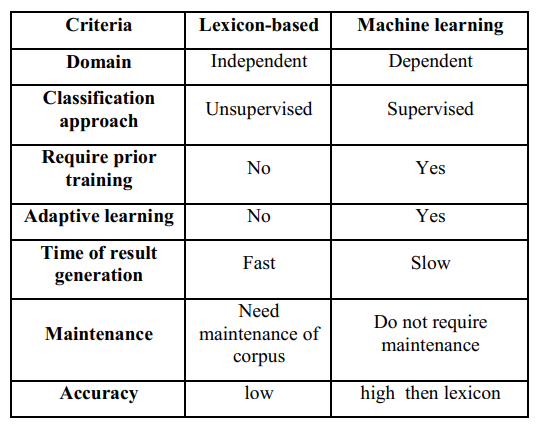
\includegraphics[width=0.5\linewidth]{images/lex_vs_ml.png}
  \caption{Comparison between lexicon and machine learning}
  \label{tab:sent_analysis_approaches}
\end{table}

Currently Sentiment analysis techniques seek to classify text as either positive, negative or neutral, using methods in Natural language processing (NLP). The common approach implemented involves statistical analysis and machine learning methods.\cite{ref2}

%
However people often express a particular emotion towards a certain topic. Specific emotions such as anger can lead to social unrest. This is undesirable but it can be helpful if we are able to quickly detect this before it occurs.
%
The proposed system will be a hybrid system it will use both machine learning approach as well as lexicon-based approach to detect both sentiment polarity and emotion.


\clearpage


\section{METHODOLOGY}
\subsection{Introduction}
In the previous chapter we explained some of the techniques which had been applied by different
researchers on sentiment analysis. The researchers tried also to explain the short comings and
strength of each technique or method applied before this research. In this chapter we are going to
explain the software and hardware development tools which we are going to use in the
implementation and development of the geographical mood detection tool. An algorithm which
the system will follow is also going to be shown in this chapter. Timely discovery of the
sentimental or opinionated web content in our case, will help the state or the government security
in the decision making, to detect sentiment of people\textquotesingle s opinions on a given topic and  to chart the results in real-time for analysis.


\begin{figure}[h]
  \centering
  \pgfimage[width=0.8\linewidth]{images/steps_to_analyse_text}
  \caption[Example figure]%
  {Steps to analyze sentiment data}
  \label{fig:ALAP:sm1}
\end{figure}




\section{Lexicon (VaderSentiment)}
A lexicon is a collection of information about the words of a language about the lexical categories to which they belong. Lexicon based sentiment analysis makes use of labeled text this is very useful in detecting sentiment by emoticons. 
%
VaderSentiment is a python library that can be used to achieve this.\\ \\
VADER (Valence Aware Dictionary and sEntiment Reasoner) is a lexicon and rule-based sentiment analysis tool that is specifically attuned to sentiments expressed in social media.
VADER makes use of sentiment lexicon, which is a list of lexical features such as words, these words are labeled according to their sentiment polarity, positive, neutral or negative.
 \\ \\
An emoticon, short for "emotion icon", also known simply as an emote, is a pictorial representation of a facial expression using characters usually punctuation marks, numbers and letters to express a person's feelings or mood, or as a time-saving method rather than to type out a whole word, an emoticon can be used to convey the writer's feelings or intended tone. \\ \\

Some key features of Vader sentiment are: -

\begin{enumerate}

\item
Punctuation: The use of an exclamation mark(!), increases the magnitude of the intensity without modifying the semantic orientation. For example, “The food here is good!” is more intense than “The food here is good.” and an increase in the number of (!), increases the magnitude accordingly.

\item
Capitalization: Using upper case letters to emphasize a sentiment-relevant word in the presence of other non-capitalized words, increases the magnitude of the sentiment intensity. For example, “The food here is GREAT!” conveys more intensity than “The food here is great!”
\item
Degree modifiers: Also called intensifiers, they impact the sentiment intensity by either increasing or decreasing the intensity. For example, “The service here is extremely good” is more intense than “The service here is good”, whereas “The service here is marginally good” reduces the intensity.
\item
Conjunctions: Use of conjunctions like “but” signals a shift in sentiment polarity, with the sentiment of the text following the conjunction being dominant. “The food here is great, but the service is horrible” has mixed sentiment, with the latter half dictating the overall rating.
\item
Preceding Tri-gram: By examining the tri-gram preceding a sentiment-laden lexical feature, we catch nearly 90\% of cases where negation flips the polarity of the text. A negated sentence would be “The food here isn’t really all that great”.
\end{enumerate}

\clearpage
\subsection{Subjectivity and Objectivity (TextBlob)}
Subjectivity and objectivity differentiates opinionated and factual based text.\cite{ref2}
Being able to detect subjectivity and objectivity is an important part of sentiment analysis, because it can tell us more about the authors emotions and intentions, a subjective person is more likely to invoke action than an objective person. TextBlob python library can be used to detect the degree of subjectivity and the degree of objectivity, these results together with the polarity scores will be used to determine the impact of the sentiment. 

\clearpage
\subsection{Multi-label convolutional neural network text classifier (Spacy)}

SpaCy is a free, open-source library for advanced Natural Language Processing (NLP) in Python \\
Spacy makes use of a neural network text classifier. SpaCy can be used to categorize documents into the different emotion classes.
The Neural network is trained using stochastic gradient descent where the estimate of the error used to update the weights is calculated based on a subset of the training dataset. \\


\begin{figure}[h]
  \centering
  \pgfimage[width=0.7\linewidth]{images/sgd}
  \caption[Stochastic Gradient decent]%
  {Stochastic Gradient decent}
  \label{fig:ALAP:sm3}
\end{figure}






A SpaCy model uses statistical decisions to make predictions, the decision is based on examples used to train the model. Training the model requires training data, training data is: examples of text with the labels that we want to predict. This will be in the following categories
\begin{itemize}
\item "anger"
\item "disgust"
\item "fear"
\item "sadness"
\item "shame"
\item "joy"
\item "guilt"
\end{itemize}




The following diagram shows how SpaCy model is trained

\begin{figure}[h]
  \centering
  \pgfimage[width=0.7\linewidth]{images/spacy_training}
  \caption[SpaCy Training]%
  {SpaCy Training:https://spacy.io/usage/training}
  \label{fig:ALAP:sm3}
\end{figure}
 
\clearpage

\subsection{Training Dataset (ISEAR)}


Robert Plutchik invented a wheel of emotions. He suggested eight primary emotions: joy opposite to sadness. Similarly, anger opposite to fear; trust opposite to disgust and surprise opposite to anticipation. These four opposite emotion pairs, show the 8 basic emotions. Additionally, Plutchik’s model shows connections between the ideas of circle of emotions using a color wheel. Like the case of colors, primary emotions can also be expressed at different degrees of their intensities, for each emotion there are three degrees. For example, serenity is a less intense degree of joy
and ecstasy is a more intense degree of joy. Plutchik’s emotions can be mixed with one another
forming a new different emotion. For example, combination of joy and trust resulted to form a new
emotion ‘love’. Likewise, joy, anger and trust are combined and form jealousy\cite{ref:4}.

\begin{figure}[h]
  \centering
  \pgfimage[width=0.5\linewidth]{images/emotion_wheel}
  \caption[Robert Plutchik's wheel of emotions]%
  {Robert Plutchik's wheel of emotions}
  \label{fig:ALAP:sm3}
\end{figure}


ISEAR (International Survey on Emotion Antecedents and Reactions) is an open dataset collected by Klaus R. Scherer and Harald Wallbott. 
ISEAR dataset contains seven major emotions based on Robert Plutchik's wheel of emotions : joy, fear, anger, sadness, disgust, shame, and guilt.\\
It has over 7,600 entries for the emotion classes. This will be a good training dataset for emotion detection.
\clearpage

\subsection{Streaming twitter (tweepy)}
Tweepy is an open source python library that can be used to stream tweets from twitter in real time through the Twitter API. The twitter api can accept parameters to filter tweets based on geolocation, language and topic (i.e. tweets containing a particular word phrase or hashtag)


\subsection{Text Processing document}
Text needs to be normalized after it is obtained,text normalization includes the following steps:
\begin{itemize}
\item converting all letters to lower or upper case
\item converting numbers into words or removing numbers
\item removing punctuations, accent marks and other diacritics
\item removing white spaces
\item expanding abbreviations
\item removing stop words, sparse terms, and particular words
\item text canonicalization
\end{itemize}

We also remove numbers since they are not relevant to our analyses. We use regular expressions to remove numbers.




\subsection{Confusion matrix}
A confusion matrix is used in machine learning to determine the performance of a classification algorithm. It is a tabular form than compares test data for which its true values are known. I will use the confusion matrix to evaluate the performance of my classification model.

A confusion matrix consists of the following classes.
 \begin{itemize}

\item
true positives (TP): This is when we have given a correct positive prediction

\item
true negatives (TN): This is when we have given a correct negative prediction.

\item
false positives (FP): This is when we have predicted yes, but the true value is no

\item
false negatives (FN): This is when we have predicted no, but the true value is yes

\end{itemize}

\begin{figure}[h]
    \centering
    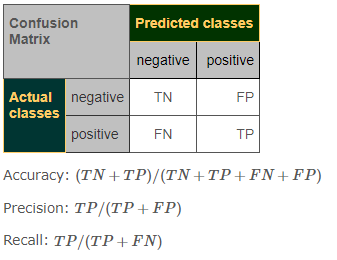
\includegraphics{images/confusion_matrix.png}
    \caption{Confusion matrix}
\end{figure}

  The above table shows how to determine the accuracy of the prediction using a confusion matrix. However, there are problems with accuracy. It assumes equal costs for both kinds of errors that is to say it assumes that we have an equal number of positives and negatives. A 99\% accuracy can either be excellent, good, mediocre, poor or terrible depending upon the problem
\clearpage
In the case of having multiple classes the confusion matrix becomes


\begin{figure}[h]
    \centering
    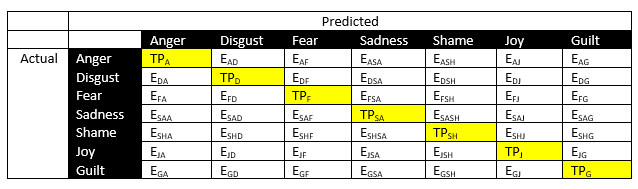
\includegraphics{images/confusion_matrix_2.png}
    \caption{Confusion matrix with multiple classes}
\end{figure}

Things to notice about a confusion matrix with multiple classes
\begin{itemize}
\item \textbf{total number of test examples} of any class if given by the sum of the corresponding row \textbf{(i.e TP + FN)}
\item \textbf{Total number of False Negatives} for a class is the sum of values in the corresponding row excluding the \textbf{True positives}

\item \textbf{Total number of false positives} for a class is the sum of values in the corresponding column excluding the \textbf{true positives}

\item \textbf{Total number of true negatives} for a certain class will be the sum of all columns and rows  excluding that classes column and row
\end{itemize}
  
\textbf{Accuracy} calculated as the sum of correct classifications divided by the total number of classifications\\
\textbf{Precision} is calculated as \textbf{ TP/(TP+ FP)}\\
\textbf{Recall} also called sensitivity, corresponds to the tue positive rate of the considered class
\\
calculated as Recall=Sensitivity=TP/(TP+FN)

\clearpage



\chapter{Implementing Sentiment analysis}

\subsection{Implementing (VaderSentiment and TextBlob)}


Using \textbf{"VaderSentiment"} library. Using an analyzer object, and looping through the list of tweets  calling the analyser.polarity\_scores() method and appending the results to an array.

\begin{lstlisting}
from vaderSentiment.vaderSentiment import SentimentIntensityAnalyzer
analyser = SentimentIntensityAnalyzer()#create the vader sentiment analyser object
sentiment_vs_tweets=[]#array will hold the processd tweets with the sentiment and objective labels
index=0
for t in tweets:
    sentiment_vs_tweets.append( analyser.polarity_scores(t) )#add the processed tweet to the list
    print(sentiment_vs_tweets[index])#print the sentiment polarity and subjecivity
    index=index+1
\end{lstlisting}


The above code will produces the following results

\begin{lstlisting}
{'neg': 0.252, 'neu': 0.581, 'pos': 0.168, 'compound': -0.3182}
{'neg': 0.0, 'neu': 1.0, 'pos': 0.0, 'compound': 0.0}
{'neg': 0.194, 'neu': 0.806, 'pos': 0.0, 'compound': -0.5574}
{'neg': 0.0, 'neu': 1.0, 'pos': 0.0, 'compound': 0.0}
{'neg': 0.194, 'neu': 0.806, 'pos': 0.0, 'compound': -0.5574}
\end{lstlisting}




Using \textbf{TextBlob} to detect the degree of subjectivity and objectivity of the documents.


\begin{lstlisting}
#here we use TextBlob python library to detect sentence/tweet/document polarity as well as subjectivity and store the results
#textblob uses a machine learning approach
from textblob import TextBlob
sentiment_tb_tweets=[]#array will hold the processd tweets with the sentiment and objective labels
index=0
for t in tweets:
    sentiment_tb_tweets.append( TextBlob(t) )#add the processed tweet to the list
    print(sentiment_tb_tweets[index].sentiment)#print the sentiment polarity and subjecivity
    index=index+1
    
sentiment_tb_tweets[0].subjectivity
\end{lstlisting}


The above code produces the following results


\begin{lstlisting}[language=Python]
Sentiment(polarity=0.0, subjectivity=0.25)
Sentiment(polarity=0.14285714285714285, subjectivity=0.31785714285714284)
Sentiment(polarity=0.0, subjectivity=0.06666666666666667)
Sentiment(polarity=0.2, subjectivity=0.2)
Sentiment(polarity=0.0, subjectivity=0.06666666666666667)
\end{lstlisting}

\clearpage

\subsection{Training SpaCy Text classifier}
Using the ISEAR training data
We can train a SpaCy model to classify text into some categories
\begin{figure}[h]
  \centering
  \pgfimage[width=0.5\linewidth]{images/isear}
  \caption{Sample ISEAR training dataset with labels}
  \label{fig:ALAP:sm1}
\end{figure}

We begin training the SpaCy model on the above training set,
start by reading in the data 
\begin{lstlisting}
nlp    = spacy.load('en_core_web_sm')#load english model
file    = open("data/train_data.txt","r")#read in training set from text file uses pipe delimiter
#read in the training set with the labels
for row in f_data:
    train_data.append( (row.split('|')[0],\
                        {"cats":\
                         {\
                          "anger"    :int(row.split('|')[1]),\
                          "disgust"  :int(row.split('|')[2]),\
                          "fear"     :int(row.split('|')[3]),\
                          "sadness"  :int(row.split('|')[4]),\
                          "shame"    :int(row.split('|')[5]),\
                          "joy"      :int(row.split('|')[6]),\
                          "guilt"    :int(row.split('|')[7])\
                        }}) )
                        
\end{lstlisting}
\clearpage
We then update the nlp model with the new training set
\begin{lstlisting}
#create the spacy nlp pipeline
textcat = nlp.create_pipe('textcat')
#add the pipeline to the nlp model| last=true since we want to add these conponents at the end of the model
nlp.add_pipe(textcat, last=True)
#declare the lables/categories
textcat.add_label('anger')
textcat.add_label('disgust')
textcat.add_label('fear')
textcat.add_label('sadness')
textcat.add_label('shame')
textcat.add_label('joy')
textcat.add_label('guilt')

optimizer = nlp.begin_training()
#next we will update the model with our own train_data from the csv file
for itn in range(1):
    for doc, gold in train_data:
        random.shuffle(train_data)
        losses = {}
        index = 0
        for text, annotations in train_data:
            nlp.update([doc], [gold], sgd=optimizer, drop=0.45, losses=losses)#drop rate at .45
            print("Iteration: {0}, %{1:.2f} Complete".format((itn+1), index/len(train_data) * 100))#show the progress
            index += 1
        print(losses)
 
\end{lstlisting}


After training the model we can now run some tweets via the model 
\begin{lstlisting}
#determine the class of the tweets using the spacy model trained earlier
#create a document and run it thru the nlp pipeline 
classified_tweets = []#array will hold the spacy classified tweets
index=0
for t in tweets:
    classified_tweets.append(  nlp(t) )
    print( classified_tweets[index].cats )#print the categories/classes of the document
    index=index+1  
\end{lstlisting}

The above code produces the following results
\begin{lstlisting}
{'anger': 0.8638094067573547, 'disgust': 0.41107258200645447, 'fear': 0.007243141997605562, 'sadness': 0.04211084172129631, 'shame': 0.7023115158081055, 'joy': 0.6675902605056763, 'guilt': 0.9010916352272034}
{'anger': 0.7449342012405396, 'disgust': 0.4830150306224823, 'fear': 0.016353892162442207, 'sadness': 0.2870638370513916, 'shame': 0.40636202692985535, 'joy': 0.1324012577533722, 'guilt': 0.41464924812316895}
{'anger': 0.7480689883232117, 'disgust': 0.4755619764328003, 'fear': 0.035106029361486435, 'sadness': 0.1592441201210022, 'shame': 0.4828783869743347, 'joy': 0.16910341382026672, 'guilt': 0.4793942868709564}
{'anger': 0.7859129905700684, 'disgust': 0.47182315587997437, 'fear': 0.026509756222367287, 'sadness': 0.32458046078681946, 'shame': 0.12689484655857086, 'joy': 0.23759214580059052, 'guilt': 0.9908844828605652}
{'anger': 0.7480689883232117, 'disgust': 0.4755619764328003, 'fear': 0.035106029361486435, 'sadness': 0.1592441201210022, 'shame': 0.4828783869743347, 'joy': 0.16910341382026672, 'guilt': 0.4793942868709564}
\end{lstlisting}

SpaCy model is able to classify the class of the text based on our training set



\clearpage

\subsection{Streaming twitter API(Tweepy)}

The python library tweepy can support accessing Twitter via Basic Authentication and the newer method, OAuth. The API parameters allow filtering tweets based on language, geolocation and tweets containing a particular word or phrase.

\begin{lstlisting}
auth   = OAuthHandler(consumer_key, consumer_secret)
auth.set_access_token(access_token, access_token_secret)

stream = Stream(auth, listner)
#run this code async 
streamer=stream.filter(track=search_terms,is_async=True,languages=langs,locations=loca_tions)
\end{lstlisting}

The listener object is a class that inherits from StreamListener class, it listens for any incoming tweets, cleans the tweets and then stores them in an array.

\begin{lstlisting}
class StdOutListener(StreamListener):
    def on_data(self, data):
        obj = json.loads(str(data))#convert the tweet into a json format
        #clean the tweets before inserting into the array
        clean_tweet = remove_pattern(obj["text"],"@[\w]*")#remove twitter handles (@user)
        clean_tweet = clean_tweet.replace("[^a-zA-Z#]", " ")#replace puntuation marks
        clean_tweet = clean_tweet.replace("RT :","")#replace the re tweet symbol
        clean_tweet = re.sub('http[s]?://(?:[a-zA-Z]|[0-9]|[$-_@.&+]|[!*\(\),]|(?:%[0-9a-fA-F][0-9a-fA-F]))+', '', clean_tweet, flags=re.MULTILINE)#remove hyperlinks
        
        score       = vs_analyser.polarity_scores(clean_tweet)
        sentiment_polarity_scores.append( float(score["compound"]) )#append the sentiment score to the array
        sentiment_tb_tweets.append( TextBlob(clean_tweet) )#append the texblob object to the array
        sentiment_vs_tweets.append( nlp(clean_tweet) )#append the vader sentiment object to the array
        tweets.append(clean_tweet)#append the clean tweet to the list of tweets
\end{lstlisting}



%%%%%%%%%%%%%%%%%%%%%%%%%%%%%%%%%%%%%%%%%%%%%%%%%%%%%%%%%%%%%%%%%%%%%%%
\subsection{Evaluating SpaCy classification model}
Because of the huge size of the training dataset, using the whole data set to train and evaluate the model would take too long. The solution therefore is to use a small sample of the dataset to train and evaluate.
The training set has 23 samples and the evaluation set has 8 samples.\\
The following is the results of the evaluation based on the confusion matrix.

\begin{lstlisting}
Accuracy:  1.4285714285714286



Precision_anger:  0.6666666666666666
Precision_disgust:  1.0
Precision_fear:  0.4
Precision_sadness:  1.0
Precision_shame:  1.0
Precision_joy:  1.0
Precision_guilt:  1.0
Total_Precision:  0.8666666666666666



Recall_anger:  1.0
Recall_disgust:  0.6666666666666666
Recall_fear:  1.0
Recall_sadness:  0.5
Recall_shame:  0.5
Recall_joy:  0.5
Recall_guilt:  0.5
Total_Recall:  0.6666666666666666
\end{lstlisting}

The results for each individual classification is quite satisfactory, considering that the training set and evaluation set is considerably small. However both the total precision and the total Recall is at least 66\% this is quite satisfactory.


\section{System design}
\subsection{INTRODUCTION}
\subsection{Purpose}
This section describes the software design and the architecture of the geographical mood detection and tool.
\subsection{Scope}
This mood detection and prediction tool will help in estimating a group of social media users'
mood toward specific topics in terms of their sentiments and opinions from their posts on twitter.\\

\subsection{System overview}
To come up with the geographical mood detection tool we utilize open source libraries, and open datasets to create models, and analyze the text then detect the mood. We will graph the results in real time then monitor the plots. From the plots we can visualize the polarity, subjectivity and emotion. We can monitor the sentiment trends in real time.

\subsection{Architectural Design}
The geographical mood detection tool, takes into consideration a number of aspects to achieve the goal namely: The sentiment polarity, degree of subjectivity, and the emotion classification. The graphical presentation of the whole system and methods to be followed are shown below:

\begin{figure}[h]
  \centering
  \pgfimage[width=0.8\linewidth]{images/system_overview}
  \caption[Example figure]%
  {System Architecture}
  \label{fig:ALAP:sm1}
\end{figure}


The first four modules describe the process implemented in order to detect mood (i.e. emotions,
speculations, evaluations and opinions) of a group of social media users through sentiment
analysis. The extracted sentiments will then help in predicting action from the group of social
media users.

\subsection{Sentiment Analysis (detection and classification)}
Once the collected corpus is clean, VaderSentiment library can be used to detect sentiment polarity the degree of positivity or negativity. Textblob library can be used to detect the degree of subjectivity or objectivity of the tweet. And SpaCy library will be used used clasisfy the emotion of the tweet.

\begin{figure}[h]
  \centering
  \pgfimage[width=0.5\linewidth]{images/sentiment_analysis_dfd}
  \caption[Example figure]%
  {Sentiment Analysis data flow diagram}
  \label{fig:ALAP:sm1}
\end{figure}


\subsection{Sequence Diagram}
The Sequence Diagram below models the collaboration of objects based on a time sequence.
It shows how the objects interact with others in a particular scenario of a use case.

\begin{figure}[h]
  \centering
  \pgfimage[width=0.5\linewidth]{images/sequence_diagram}
  \caption[Example figure]%
  {Illustration of the Sequence diagram}
  \label{fig:ALAP:sm1}
\end{figure}


\subsection{Use Case Diagrams}
\textbf{Blogger}\\
Bloggers from all over the world interact through social media platforms by commenting and
uploading posts part of our tool\textquotesingle s task is to crawl on these platforms for text related to a searched term. 



\begin{figure}[h]
  \centering
  \pgfimage[width=0.5\linewidth]{images/use_case_blogger}
  \caption[Example figure]%
  {Blogger use case diagram}
  \label{fig:ALAP:sm1}
\end{figure}

\clearpage
\textbf{User}\\
A user of the system may input a \textbf{keyword/phrase} that will be searched on the social media platforms which will help in mining content concerning the searched keyword. Furthermore, user has the
flexibility of changing keyword search parameters.

\begin{figure}[h]
  \centering
  \pgfimage[width=0.5\linewidth]{images/system_user_use_case}
  \caption[Example figure]%
  {System user use case diagram}
  \label{fig:ALAP:sm1}
\end{figure}



\section{Development Tools}

\subsection{SpaCy}

\begin{minipage}{0.4\textwidth}
\begin{itemize}
\item[\textbf{\emph{}}] 
SPaCy is an open source python library used for common NLP tasks. The library implements statistical neural network models, it has language support for English, German, Spanish, Portuguese, French, Italian, Dutch as well as tokenizations for various other languages.
\end{itemize}
\end{minipage}%
%
\begin{minipage}{0.4\textwidth}
\begin{center}
    
\includegraphics[width=0.6\textwidth]{images/spacy_logo}
    %\captionof{figure}{Gripper}
    \label{img:g}
\end{center}
\end{minipage}




\subsection{VaderSentiment}
\begin{minipage}{0.4\textwidth}
\begin{itemize}
\item[\textbf{\emph{}}] 
VaderSentiment is a python library built on top of NLTK. it is a rule-based sentiment analysis engine, and implements grammatical and syntactical rules to detect sentence polarity, positive, negative and neutral.
\end{itemize}
\end{minipage}%
%
\begin{minipage}{0.4\textwidth}
\begin{center}
    
\includegraphics[width=0.5\textwidth]{images/VaderSentiment_logo}
    %\captionof{figure}{Gripper}
    \label{img:g}
\end{center}
\end{minipage}



\subsection{TextBlob}
\begin{minipage}{0.4\textwidth}
\begin{itemize}
\item[\textbf{\emph{}}] 
TextBlob is a python library for processing textual data. TextBlob can be used to determine the degree of subjectivity or objectivity in a textual document.
It provides a simple API for diving into common natural language processing (NLP) tasks such as part-of-speech tagging, noun phrase extraction, sentiment analysis, classification, translation, and more.\cite{ref43}
\end{itemize}
\end{minipage}%
%
\begin{minipage}{0.4\textwidth}
\begin{center}
    
\includegraphics[width=0.5\textwidth]{images/textblob_logo}
    %\captionof{figure}{Gripper}
    \label{img:g}
\end{center}
\end{minipage}


\subsection{Jupyter Notebook}
\begin{minipage}{0.4\textwidth}
\begin{itemize}
\item[\textbf{\emph{}}] 
The Jupyter Notebook App is a server-client application that allows editing and running notebook documents via a web browser. The Jupyter Notebook App can be executed on a local desktop requiring no internet access or can be installed on a remote server and accessed through the internet.\cite{ref46}
\end{itemize}
\end{minipage}%
%
\begin{minipage}{0.4\textwidth}
\begin{center}
    
\includegraphics[width=0.5\textwidth]{images/jupyter_notebook}
    %\captionof{figure}{Gripper}
    \label{img:g}
\end{center}
\end{minipage}






\subsection{MatplotLib}
\begin{minipage}{0.4\textwidth}
\begin{itemize}
\item[\textbf{\emph{}}] 
Matplotlib is a plotting library for the Python programming language and its numerical mathematics extension NumPy. It provides an object-oriented API for embedding plots into applications using general-purpose GUI toolkits like Tkinter, wxPython, Qt, or GTK+.\cite{ref45}
\end{itemize}
\end{minipage}%
%
\begin{minipage}{0.4\textwidth}
\begin{center}
    
\includegraphics[width=0.5\textwidth]{images/matplot_lib}
    %\captionof{figure}{Gripper}
    \label{img:g}
\end{center}
\end{minipage}



\section{Creating Twitter Application}
Navigate to the url \url{https://developer.twitter.com/en}\\
under the "App Details" tab fill in your application details and move to the next tab "Keys and Tokens"

\begin{figure}[h]
  \centering
  \pgfimage[width=0.6\linewidth]{images/twitter_1}
  \caption[Example figure]%
  {Application Details}
  \label{fig:ALAP:sm1}
\end{figure}

Collect the keys, secret key and API key which will be used by the tweepy library for authentication and streaming tweets.


\begin{figure}[h]
  \centering
  \pgfimage[width=0.6\linewidth]{images/twitter_2}
  \caption[Example figure]%
  {Access keys}
  \label{fig:ALAP:sm1}
\end{figure}

\clearpage
Set the permissions for your API key.


\begin{figure}[h]
  \centering
  \pgfimage[width=0.5\linewidth]{images/twitter_3}
  \caption[Example figure]%
  {API permissions}
  \label{fig:ALAP:sm1}
\end{figure}



\section{Implications of findings}
The boom in the availability of opinionated and emotionally charged data from various
review sites, RSS feeds, and social networks has created a wave of interest in sentiment analysis
by both academia and businesses. This is because there are many practical and potential
applications of sentiment analysis. A Geographical Mood Detection tool can
assist organizations and service providers to know the mindset of the people they are working
with for instance:\\

\textbf{Business Applications}\\
The tool can be adopted by any business which would like the ability to exploit unstructured data for actionable insights. Potential applications would be extracting product review, brand tracking, modifying
marketing strategies and mining financial news.\\

\textbf{Politics}\\
Sentiment analysis enables tracking of opinion on issues and subjectivity of bloggers in
political blogs. Sentiment analysis can help political organization to understand which issues
are close to the voter\textquotesingle s heart.\\

\textbf{Government Intelligence}\\
For efficient rule making, the tool can be used to assist in automatically analyzing the opinions of
people about pending policies or government-regulation proposals. Other applications include
tracking the citizen\textquotesingle s opinion about a new scheme, predicting the likelihood of the success of a new legislative reform to be introduced and gauging the mood of the public towards a scandal
or controversy.



\chapter{RECOMMENDATIONS, FUTURE WORK AND CONCLUSION}
\subsection{Recommendations}
This tool may be used by the government, Non-Governmental Organizations, and business
corporations. Investors may need to analyze the environment first before starting a business
venture, hence detecting mood of a society concerning a particular topic/product is of vital importance.
We also propose that the tool can be used with experts in the field of big data analytics so as to gain
better insights into their business/political atmosphere. It is clear that the adoption of advanced analytic approaches such as those used by our tool can guide organization\textquotesingle s to  strategize and help them to make smarter decisions.\\

\subsection{Future Work}
In future work we plan to devise an approach to further improve the accuracy of mood detection by including not only textual information but also pictorial, video, and audio classification.
Having said that, we believe that sentiment analysis will only increase in importance as more and
more people use online channels to communicate, both directly and indirectly.
We also plan to consider the issue of sarcasm, that is, sarcastic sentences express negative opinion
about a target using positive words. For example:\\

$\cdot$ “Nice perfume. You must marinate in it”.\\
The sentence contains only positive words, yet still, it expresses a negative sentiment.






\chapter{Results and analysis}\label{ch:Results}
\section{Data visualization}
Because of the way the human brain processes information, using charts or graphs to visualize large amounts of complex data is easier than poring over spreadsheets or reports. 
Data visualization makes it easier to identify areas that need attention.

\subsection{matplotlib and seaborn}
Seaborn is a Python data visualization library based on matplotlib. It provides a high-level interface for drawing attractive and informative statistical graphics.
Matplotlib allows plotting multiple graphs on a single figure. Analysis can be made on different metrics at the same time. It also allows updating graph data in realtime.
\clearpage
\begin{figure}[h]
  \centering
  \pgfimage[width=0.5\linewidth]{images/graphs_results}
  \caption[Real time plot of the analysis]
  {Real time plot of the analysis}
  \label{fig:ALAP:sm1}
\end{figure}


The \textbf{wordcloud} gives a summary of the tweets in realtime.\\
The \textbf{timeseries} gives a \textbf{stochastic trend} of the polarity of the tweets, with \textbf{1 = positive, -1 = negative and 0 = neutral}.
The \textbf{barchart} displays the values of the number of tweets in the given category\\
The \textbf{heat map} shows the \textbf{polarity} as well as the \textbf{subjectivity} in terms of percentage,
a negative and subjective scenario is the least desirable while a positive and objective scenario is the most desirable.\\

With this realtime analysis one can quickly see the prevailing mood as well as a summary of the tweets around a given topic.





\chapter{Conclusion}
This research project has examined the role of social media networks in determining peoples mood based on textual information they post. We developed a geographic mood detection tool based on social media.

The results show that by utilizing social media platforms e.g. twitter, a tool can actually analyze peoples mood towards a subject and inform the relevant authorities in real-time to know what the people\textquotesingle s general mood towards a particular subject is.

Making use of open python libraries and training data sets we were able to classify the general mood 
of people based on their geographical location.

Furthermore, this tool can be adopted by businesses, organizations and politicians who would like to have an edge and an insight into peoples opinions over a giver topic.


















